\documentclass[runningheads]{llncs}
%
\usepackage{algorithm}
\usepackage{amsmath}
\usepackage{amssymb}
\usepackage{algpseudocode}
\usepackage{graphicx}
% Used for displaying a sample figure. If possible, figure files should
% be included in EPS format.
%
% If you use the hyperref package, please uncomment the following line
% to display URLs in blue roman font according to Springer's eBook style:

%\hypersetup{
%   colorlinks=false,
%  pdfborder={0 0 0},
%}
\usepackage{hyperref,xcolor}% http://ctan.org/pkg/{hyperref,xcolor}
\usepackage{makeidx}
\definecolor{winered}{rgb}{0.5,0,0}
  
\hypersetup
{
    pdfauthor={Anurag Dutta},
    pdfsubject={Hyperlinks in LaTeX},
    pdftitle={myhyper.tex},
    pdfkeywords={LaTeX, PDF, hyperlinks}
%    colorlinks=false,
    pdfborder={0 0 0},
%You can set individual colors for links as below:
colorlinks=true,
 linkcolor=winered,
urlcolor={winered},
filecolor={winered},
%citecolor={winered} %Gives errors when turned on
%allcolors={winered} %Gives errors when turned on
  linktoc=all,
}
\begin{document}
%
\title{Linguistic Exploratory Data Analysis \textit{vis-à-vis} Shri Bhagavad Gita}
%
%\titlerunning{Abbreviated paper title}
% If the paper title is too long for the running head, you can set
% an abbreviated paper title here
%
\author{Anurag Dutta\inst{1}\orcidID{0000–0002–5787–3860}}
%
\authorrunning{A. Dutta et al.}
% First names are abbreviated in the running head.
% If there are more than two authors, 'et al.' is used.
%
\institute{Undergraduate, Department of Computer Science, Government College of Engineering and Textile Technology, Serampore, Calcutta, India \\\textbf{\\}
\email{anuragdutta.research@gmail.com}\\
}
%
\maketitle              % typeset the header of the contribution



%%==================================%%
%% sample for unstructured abstract %%
%%==================================%%
\begin{abstract}
Both eastern and western experts agree that the Bhagavad-Gita is one of the finest philosophical works yet written. The Ultimate Lord Krishna explains the art of consciousness and the precise procedure through which a person might forge an enduring bond with God in a manner that is both amazing and quite obvious. The Bhagavad Gita is unparalleled in regards to pure, spiritual discernment. Its inherent beauty is that it does not presuppose any religious ideology or secular viewpoint and that its knowledge is applicable to all people. It is revered as the pinnacle of all spirituality and is approachable from the holy spheres of all faiths. In this article, we would perform an Exploratory Data Analysis on the Bhagavad Gita in chapter wise manner. Further, we would root down the phrases in the Bhagavad Gita with maximal count.  The same was done in both Chapter Wise manner, and also for the entire Script of Shri Bhagavad Gita. An eclectic topic within linguistics, information science, and machine intelligence called "Natural Language Processing" studies ways machines and modern speech engage, with either a focus here about how to design machines to gather and analyse massive quantities of natural textual information. We would make use of Natural Language Processing for the Exploratory Data Analysis. 
\end{abstract}


\section{Introduction}\label{sec1}
One of India's early literature, the \textit{Bhagavad Gita}, was developed out from \textit{Mahabharata}, an epigram. With more than 100,000 \textit{Shlokas}, or more than 200,000 syllables, this hymn continues to hold the record for being the longest ballad ever composed thru history. The \textit{Bhagavad Gita} represents merely a portion of this enormous work, but it is arguably among the most significant and beloved \textit{Vedic} scriptures ever produced. This enormous poem includes literature like Upanishads as well as the \textit{Dhammapada}, but it is \textit{Bhagavad Gita} that would be frequently recognised as being the one that possesses the key to development of quality. \\\textbf{\\}

The \textit{Bhagavad Gita}'s overall narrative actually took place mostly on \textit{Kurukshetra} battleground, where two rival families the \textit{Pandavas} and even the \textit{Kauravas} are getting ready to go to war. The dialogue amongst \textit{Krishna} \& \textit{Arjuna} serves as the central focus of the work. The \textit{Bhagavad Gita}, also known as the "\textit{Song of the Lord}," is one of many literature from this historical era which, much like \textit{Upanishads} and also the \textit{Dhammapada}, appears to be almost eternal in the sense that it still important now just as it was a thousands of years ago. We investigate on which transpires when \textit{Arjuna} must make crucial decisions that affect the trajectory of his life, particularly the choice whether or not to engage in combat with representatives of his own clan in a conflict between "good" and "bad," as well as the significance of leading a life of integrity and meaning. The \textit{Bhagavad Gita}'s tokenistic and metaphorical nature makes it one of the most fascinating and sometimes misunderstood aspects of \textit{Hinduism}. The actual text is a reflection of the struggle that takes place in our thoughts and serves as an excellent tool to comprehend how we might get through hardship and self-doubt but also, in the end, how and where to live an existence of honesty and significance. There is no actual battle or war to be conquered. The Bhagavad Gita delves deeper into the concept of "Dharma," that refers as "that which supports" and is frequently referred to as "life purpose." It is reported that great writers including \textit{Beethoven}, \textit{John Keats}, \textit{Walter Hagan}, and \textit{Henry David Theroux} having found solace and direction in the \textit{Bhagavad Gita}'s chapters. There are 18 chapters in the \textit{Bhagavad Gita}.  \\\textbf{\\}

For several explanations, Natural Language Processing constitutes one of the most significant branches of cognitive computing. Its most conventional thing for a client and a system to communicate is through Natural Speech. This ideally includes Voice Synthesis and Speech Comprehension. Although \textit{Alan Turing} acknowledged this in his essay on "consciousness," where he established the "Turing Test" like a method for determining if a system is capable of displaying cognition through a dialogue in Natural Speech. The substantial majority of textual information that exists throughout the globe and serves as a catalyst for Natural Language Recognition and Comprehension is one of the main advantages of Natural Language Processing transcend Voice - Recognition innovation. We might open up a tonne of potential functions for upcoming machine learning purposes and a tonne of expertise that may be placed to use if a computer could analyze, organise, and comprehend this language. The broad spectrum of employing Natural Language Processing serves as evidence of its significance. The much more intuitive way to interact with machines and the vast amount of unorganized data that is available digitally is through Natural Language Processing. This article incorporates NLP for Exploratory Data Analysis of the \textit{Bhagavad Gita}. 
\section{Shri Bhagavad Gita}
The Gita is structured as a series of conversations featuring Pandava prince Arjuna \& his charioteer and mentor Krishna. Arjuna is distracted with a moral and psychological conflict at the beginning of the just conflict seen between Pandavas and indeed the Kauravas and is depressed about the brutality and deaths the conflict would bring about in the struggle versus his relatives. Geeta has a total of 700 verses and 18 chapters.
\subsection{Chapter 1: Arjuna Vishada Yoga}
\textit{King Dhritarashtra}, who is blind, requests that the poet \textit{Sanjaya} narrate the account of his ancestors, the \textit{Kurus}, engaging the \textit{Pandavas} in combat. \textit{Sanjaya} recounts how Prince \textit{Duryodhana}, the son of \textit{King Dhritarashtra}, asked his instructor \textit{Drona} to have a glance at the gathered soldiers. \textit{Duryodhana} draws attention to the powerful and imposing members of \textit{Pandava} army, including \textit{Arjuna} and \textit{Krishna}. He then goes to the influential figures in his own legion, praising some of them as outstanding fighters. \textit{Duryodhana} boasts that the \textit{Kuru} cavalry is insurmountable while the \textit{Pandavas'} army is considerably smaller. Calling the soldiers to battle, both battalions burst conch shells that resound "throughout heaven and earth." In order for them to appear between the two armies, \textit{Arjuna} commands \textit{Krishna} to steer the chariot carrying them. He want "to view the men assembled to perform military duty for \textit{Dhritarashtra}'s wicked son." \textit{Krishna} draws \textit{Arjuna}'s awareness to all of the \textit{Kurus} who are prepared for combat. Looking out at the rival factions made out of his kin, \textit{Arjuna} is overcome with terror. He informs \textit{Krishna} that he perceives "bad omens from slaying my kinsmen in combat," and that he does not wish to fight his family, even if they are enemies. \textit{Arjuna} advises \textit{Krishna} that it would be preferable for him to surrender in the combat than to take part in this horrible conflict. 
\subsection{Chapter 2: Sankhya Yoga}
Such shyness at this time, \textit{Krishna} answers to \textit{Arjuna}, is "contemptible of a noble soul." \textit{Arjuna} continues to say that he is unable to stand the idea of murdering his relatives. In verses 11–17, Krishna emphasises that physical sensations are ephemeral, just the same as death and life were, and that \textit{Arjuna}'s "grief is utter misconception" because of this. Everything that is here now has always been here. Every life, \textit{Arjuna} and his clan will simply transition from one physique to the next. Since his "Self" is everlasting and a component of the everlasting tapestry of the cosmos, \textit{Krishna} exhorts \textit{Arjuna} to fulfil his obligations in this lifetime. \textit{Arjuna} cannot actually murder or be killed as only the physical may pass away. \textit{Krishna} asserts in verse 31 that \textit{Arjuna}'s mission in this incarnation is to be a warrior. \textit{Arjuna} therefore must carry out that obligation in order to live up to his full potential. \textit{Krishna} cautions against focusing too much on the literature rather than using contemplation to free the consciousness of uncertainty and craving. Action must be taken solely for its own purpose and not because of any connection to the outcomes. \textit{Krishna} teaches that this is the karma yoga method of life. \textit{Krishna} responds to \textit{Arjuna}'s question about how a wise man operates in the universe by saying that a wise man immerses himself in contemplation and manages to disengage from the overstimulation of the outside world.
\subsection{Chapter 3: Karma Yoga}
\textit{Arjuna} is perplexed and wonders why \textit{Krishna} seems to promote the way of wisdom and understanding while pressuring \textit{Arjuna} to take action. The two paths are awareness and conduct, \textit{Krishna} continues. Some individuals are more suitable suited for the first pathway than others. According to \textit{Krishna}, performing required and righteous deeds is another type of worship and the Self can only be released by doing so. The moral behaviour of "great men" also establishes a standard for regular people to aspire to. Krishna observes that while having no needs or desires, he yet does action. If he stopped, humanity would imitate him and succumb to the trap of passivity. \textit{Krishna} further exhorts \textit{Arjuna} to remove the egotistical "I" from his deeds and steer clear of the fallacy that "I am the doer" of each and every deed. \textit{Arjuna} must realise that every conduct is really just the \textit{gunas} interacting on upon \textit{gunas}. Then \textit{Arjuna} queries \textit{Krishna} about the motivations behind men's wicked deeds. \textit{Krishna} adds that they are motivated by the trait known as \textit{rajas}, which encompasses passion and aggression. When this \textit{guna} is present in excess, it drives individuals to behave out of resentment and willingness, which leads to wicked deeds. \textit{Krishna} maintains that in order to prevent this, the intellect has to be powerful than the perceptions and self-awareness must be better than the intellect.
\subsection{Chapter 4: Jnana-Karma-Sanyasa Yoga}
\textit{Krishna} explains to \textit{Arjuna} that he is giving him a timeless lesson. Although \textit{Krishna} had previously imparted this knowledge to deities as well as other beings preceding \textit{Arjuna}, it has since been forgotten and degraded. \textit{Arjuna} wonders if the fact that \textit{Krishna} was born in the late than that of the sun deity could explain this loss. \textit{Krishna} explains that he is everlasting, has many births, and manifests as a human being when purity wavers. \textit{Krishna} is present in this form to assist \textit{Arjuna} in comprehending the nuanced essence of conduct. \textit{Krishna} states that when someone worships God, God serves as both the performer and the action in this situation. There are several ways to do devotion or commitment, including as via contemplation, consciousness, and biblical learning.
\subsection{Chapter 5: Karma-Sanyasa Yoga}
\textit{Arjuna} questions \textit{Krishna} about which path—renunciation or active engagement preferable for him. \textit{Krishna} responds that while both routes are worthwhile, the karma yoga route is much more straightforward. If thoroughly cultivated, both the path of abstinence and the road of engagement lead to the Absolute. The knowledgeable philosopher and the practitioner of karma yoga simultaneously engage in conduct, whether that be physical activity in combat or mental action while contemplating the texts, sans commitment to the outcomes. Men "act badly" because they lack self-awareness. Knowing that the Absolute at the centre of every creature is identical and is just clothed in various bodies, \textit{Krishna} emphasizes that "intelligent folks view all beings as similar."
\subsection{Chapter 6: Atma-Samyama Yoga}
\textit{Krishna} claims that since doing the right thing, or practising karma yoga, necessitates surrender of one's "own selfish will," it is likewise renunciation. A individual who has previously accomplished those things can help their soul by using their self, which consists of their thoughts, perceptions, and body. The very same self that prevents someone from recognising their own inner Self is also that self. Instead of exercising self-control over the intellect, physique, and perceptions, some individuals choose to let them rule themselves. One needs to become an expert in meditation in order to practise yoga. This method entails sitting in a spotless region surrounded by a rag, focusing on a "single item," maintaining a straight spine, and being frugal with both sleep and food. The mind becomes tranquil and peaceful during meditation, and as a result, it melts to disclose the One. Through meditating and practicing yoga, one can liberate one's oneself of pain or discomfort.
\subsection{Chapter 7: Jnana-Vijnana Yoga}
\textit{Krishna} promises to teach to \textit{Arjuna} how cultivating nonattachment enables one to know God. Krishna subsequently concentrates on explaining to \textit{Arjuna} how God is the essential nature of the cosmos and that his present form is merely a reincarnation on earth. \textit{Krishna} claims that almost all people are unable to comprehend how he is the essential component of all phenomena. Individuals who lack knowledge are seduced by \textit{Krishna}'s strength and everything he has made visible to them. Others, nevertheless, are able to see through the threefold \textit{gunas }and comprehend that God is the unchanging substance of everything. \textit{Krishna} categorises his devotees into four groups: the sage, the individual in need, the power-seeker, and the wisdom-seeker.
\subsection{Chapter 8: Aksara-ParaBrahma Yoga}
\textit{Krishna} helps \textit{Arjuna} comprehend the nature of existence and how reincarnation and liberation from the reincarnation cycle are related. Again, there is a sophisticated understanding behind the interchangeable usage of phrases like Supreme Person, God, \& \textit{Krishna}. Yoga practitioners think about how the One and God are eternal souls who exist outside of the physical, intellect, and emotions. That individual will achieve liberation by concentrating on this greatest soul, or Krishna.
\subsection{Chapter 9: Raja-Vidya-Raja-Guhya Yoga}
\textit{Arjuna} has confidence in \textit{Krishna}. \textit{Krishna} offers to reveal to \textit{Arjuna} the method for gaining wisdom and finding relief from suffering in exchange. The boundless, transcendental form of \textit{Krishna} contains all life forms, but \textit{Krishna} also isn't constrained by them. At the beginning and the end of the celestial cycles, he is unconcerned with the results of creation. \textit{Krishna} is undisturbed whether all entities are brought forth at the beginning of the cycle or are gathered back to him at its conclusion. He is not a part of any action. People who worship other deities are really worshipping the creator of all reality, \textit{Krishna}, in his uncreated state. They are not conscious of this, thus when \textit{Krishna} assumes physical figure, they do not acknowledge or respect him.
\subsection{Chapter 10: 	Vibhuti Yoga}
\textit{Arjuna} is still being taught by \textit{Krishna} about what it means to be the greatest incarnation of God. In light of this, \textit{Krishna} appears as every other gods and spiritual figures. He cites instances like the lightning deity \textit{Indra} pretending to be \textit{Indra} and the lightning bolt of \textit{Indra}. \textit{Krishna} claims that he is both the good and bad aspects of the universe, including both joy and suffering, bravery and fear. A person will be released from the reincarnation cycle if they can imagine \textit{Krishna} as the origin of all appearances. A wise man achieves oneness with God through meditation. This is a type of worship, says \textit{Krishna}. Entering a condition of divinity and realising knowing \textit{Krishna} is the wellspring is the ultimate form of devotion.
\subsection{Chapter 11: Viswarupa-Darsana Yoga}
After finally grasping a large portion of \textit{Krishna}'s message, \textit{Arjuna} requests that \textit{Krishna} reveal his "ultimate form." According to the poet \textit{Sanjaya}, \textit{Krishna} reveals to \textit{Arjuna} the immensity and majesty of his presence by revealing to him the "whole cosmos enshrouded in the torso of the God of gods." The vision is especially horrifying since it shows \textit{Krishna}'s self as having a vast array of heads, claws, and weaponry. The image humbles and astounds \textit{Arjuna}. He recounts his observations, which include a glimpse of Krishna consuming every one of the \textit{Kauravas}.
\subsection{Chapter 12: Bhakti Yoga}
\textit{Arjuna} poses the chapter's central dilemma by pondering whether it is preferable to have religious affection for the more intangible, transcendental God or for \textit{Krishna}. Both paths will ultimately to enlightenment, \textit{Krishna} responds, but corporeal people should choose the path of passionate adoration for \textit{Krishna} as he is personified in the \textit{Gita}. According to him, praising \textit{Krishna} in this physical form helps devotees maintain their attention. Though it takes more effort, honoring the enormous God as the principle that permeates everything will surely bring followers to insight. \textit{Krishna} insists that the only way to reach him is to focus solely on him during meditation. If such concentration is not feasible, then an individual will ultimately meet \textit{Krishna} by leading a life that is dedicated to him.
\subsection{Chapter 13: 	Ksetra-Ksetrajna-Vibhaga Yoga}
\textit{Krishna} asserts that physical sensations like heat or cold are caused by the natural world. Reactions to body composition, such as discomfort and pleasure, are produced by the Individual. Both are "without beginning" and are acts of God. A person's biological predisposition affects how they connect with environment, determining whether they are happy and affectionate enthusiastic and energetic, or gloomy and pessimistic. The bodily effort that gives humanity and all of its chaos its form is created by nature. The nature experience and the physique, with their corresponding pleasant and unpleasant emotions and sensations, are nevertheless separate from the Self. Being aware of this distinction will enable one to break the chains from the reincarnation cycle.
\subsection{Chapter 14: Gunatraya-Vibhaga Yoga}
\textit{Arjuna} is given instructions by \textit{Krishna} regarding the pinnacle of knowledge attained by yoga gurus. He emphasizes that nature is "the womb" and that he is "the seed-giving father." All living things are the result of the union of the two. \textit{Sattva}, \textit{rajas}, \& \textit{tamas} are the three \textit{gunas}, and they are determined by a person's temperament. The \textit{gunas} maintain the everlasting Self's corporeal body-bound status. \textit{Rajas} and \textit{Tamas} are bound by desire and exertion, while \textit{Sattva} and \textit{Rajas} and \textit{Tamas} are bound by sloth and slumber. Since \textit{sattva} is associated with wisdom, it has the ability to elevate an individual and bring about awareness. The other two either drag a man down or cause immobility.
\subsection{Chapter 15: Purushottama Yoga}
\textit{Krishna} compares "the domain of sorrow" to a tree, whose roots are action and whose branches are the \textit{gunas}. The religious melodies are represented by the foliage. \textit{Arjuna} is told by \textit{Krishna} to chop down this tree "with the sharp-edged axe of detachment" and look for God, also known as "the original Person," who is the source of the cosmos. When \textit{Krishna} dwells a body, he appreciates its feelings and allows them flow like smells on the breeze rather than becoming addicted to them. Those who practise self-control and the yoga path are able to recognise God as their own Self.
\subsection{Chapter 16: Daivasura-Sampad-Vibhaga Yoga	}
\textit{Krishna} contrasts "those with demonic tendencies" with "intelligent men" by describing their attributes. The qualities of a sage or an enlightened person are considered to be divine qualities. Purity of spirit, honesty, empathy, bravery, and a generous spirit are some examples of these qualities. Krishna views arrogance, wrath, dishonesty, and illiteracy as evil attributes. \textit{Krishna} claims that \textit{Arjuna }possesses the qualities of the gods. A guy born with demonic tendencies may believe "the universe has no moral, no truth, no God," according to \textit{Krishna}. By allowing oneself to be ruled by their never-ending cravings, these individuals join hell. These guys are conceived repeatedly into "demonic wombs," and as a result, they are imprisoned in hell.
\subsection{Chapter 17: Shraddhatraya-Vibhaga Yoga}
\textit{Om Tat Sat} is explained by \textit{Krishna}. \textit{Om} is a sacred sound that is repeated before doing acts of worship, control, or charity. \textit{Tat}, which means "the Absolute" in Sanskrit, is repeated upon doing the correct thing. Chanting \textit{Sat} denotes a "praiseworthy action." Sanskrit terms such as \textit{asat}, or "unreal," are used to describe acts of worship, control, or generosity that are carried out without faith.
\subsection{Chapter 18: Moksha-Sanyasa Yoga}
The final sentence of the chapter emphasises the importance of devotion to \textit{Krishna} for a yoga practitioner. He advises \textit{Arjuna} to put \textit{Krishna} at the centre of his attention and to stop worrying. As a result, \textit{Arjuna} will be saved. Anyone who has a complete devotion to \textit{Krishna} is going to be liberated in this manner. The individuals who are committed and working towards God are the only ones who have access to \textit{Krishna}'s secret. \textit{Arjuna} pledges to battle and conveys his utmost appreciation to \textit{Krishna} for teaching him the reality. \textit{Sanjaya}, a poet, has finished presenting the most hidden philosophy that he learned straight from \textit{Krishna}. In his final statement, he asserts that righteousness and intellectual prosperity are present wherever the "Lord of Yoga" and "\textit{Arjuna }the archer" reside.
\section{Exploratory Data Analysis}
As a strata of the EDA, we would firstly, start off with counting the number of Verses for each Chapter. Figure \ref{fig1} demonstrates the Chapter Wise Verse Count for Shri Bhagavad Gita
\begin{figure}
\centering
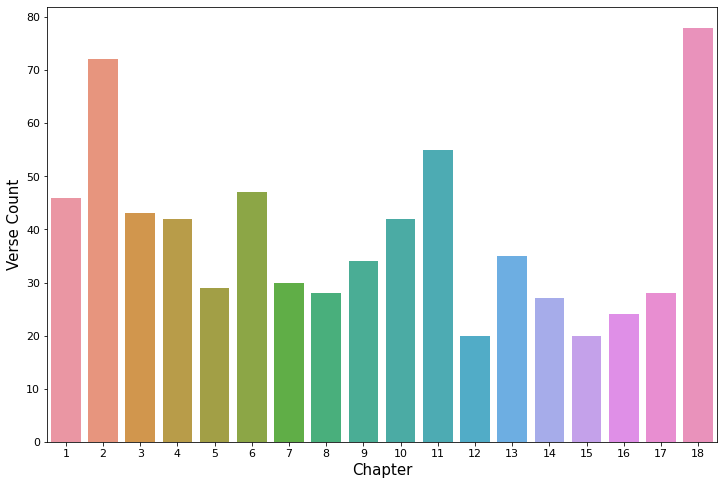
\includegraphics[width=\textwidth]{1}
\caption{Graphical Representation of the number of Verse for each Chapters of the Bhagavad Gita}
\label{fig1}
\end{figure} 
Figure \ref{fig1} demonstrates that the Chapter 18 of the Bhagavad Gita is having the maximal number of the Verse (78), followed by Chapter 2 (72). In total, there are 700 verses in the Gita. A tag cloud, commonly referred to as a Word Cloud, is a graphical portrayal of text data that is frequently used to show free-form text or keyword information on internet sites. Tags are often words or phrases, and the text size or colour of each indicates its significance. Figure \ref{fig2} demonstrates the Word Cloud of the Bhagavad Gita.
\begin{figure}
\centering
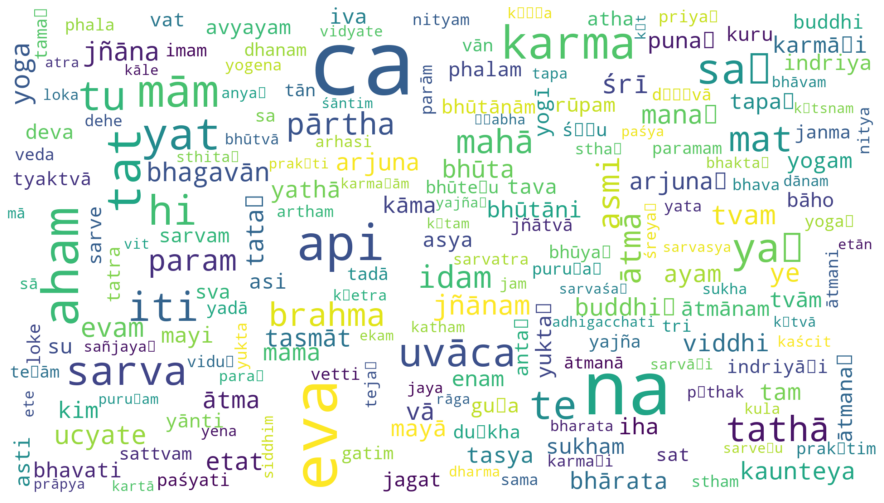
\includegraphics[width=\textwidth]{2}
\caption{WordCloud of Shri Bhagavad Gita. Size of word in the cloud signifies their frequency. }
\label{fig2}
\end{figure} 
The most prominent words being $\mathtt{parth}$, $\mathtt{uvaca}$, $\mathtt{karma}$, etc. 
Chapterwise WordCloud can be visualized from \href{https://github.com/Anurag-Dutta/Linguistic-Exploratory-Data-Analysis-vis---vis-Shri-Bhagavad-Gita}{https://github.com/Anurag-Dutta/Linguistic-Exploratory-Data-Analysis-vis---vis-Shri-Bhagavad-Gita}. 
\end{document}